%!TEX TS-program = xelatex

\documentclass[]{friggeri-cv}
\usepackage{ctex}
\usepackage{afterpage}
\usepackage{hyperref}
\usepackage{color}
\usepackage{xcolor}
\hypersetup{
    pdftitle={},
    pdfauthor={Feng},
    pdfsubject={},
    pdfkeywords={resume},
    colorlinks=false,       % no lik border color
   allbordercolors=white    % white border color for all
}
\addbibresource{bibliography.bib}
\RequirePackage{xcolor}
\definecolor{pblue}{HTML}{0395DE}
%header
\begin{document}
\header{上海}{XXX}
      { 彭峰 } 
      
 %对应cls中的  node的三个   

% Fake text to add separator      
\fcolorbox{white}{gray}{\parbox{\dimexpr\textwidth-2\fboxsep-2\fboxrule}{%
.....
}}


\begin{aside}
  \section{工作意向}
    运维开发工程师
    ~
  \section{Phone \& Skype}
    17091314725
    ms6577
    ~
  \section{Email}
    \href{mailto:git4xuan@gmail.com}{\textbf{git4xuan@}\\gmail.com}
    \href{mailto:jobs@fengidea.com}{\textbf{jobs@}\\fengidea.com}
    ~
%  \section{在线简历}
%    \href{http://devops.mxuan.me}{devops.mxuan.me}
%    \href{https://bitbucket.org/neoben}{bitbucket.org/neoben}
%    \href{https://github.com/neoben}{github.com/neoben}
    ~
  \section{Language}
    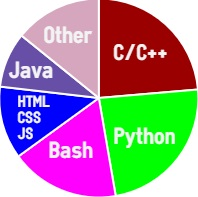
\includegraphics[scale=0.72]{img/programming.jpg}
    ~
  \section{OS Preference}
    \textbf{openSUSE}
\includegraphics[scale=0.40]{img/5stars.png}
    \textbf{Debian}
\includegraphics[scale=0.40]{img/4stars.png}
    \textbf{CentOS}
\includegraphics[scale=0.40]{img/3stars.png}
    \textbf{Windows}
\includegraphics[scale=0.40]{img/3stars.png}
    ~
  \section{Personal Skills}
    ~
    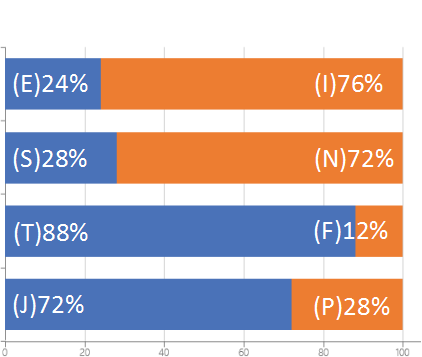
\includegraphics[scale=0.72]{img/personal.png}
    ~
\end{aside}

\section{项目介绍}
\begin{entrylist}
  \entry
    {02/15 - 05/15}
    {嵌入式显微成像系统}
    {Qt5 Django }
    {在树莓派的基础上搭建的系统平台,在嵌入式系统下对光学薄膜进行数字显微成像和基本的图像处理,并可以远程显示和控制。同时利用Gentoo,可以对内核进行系统精简实现集成化。
     硬件部分包括了光学衔接系统、显微采集硬件模块设计、光源设计;%摄像头驱动编写,
     经过图像锐化和降噪处理后的图像可以在C++编写的远程控制软件(Qt5)和Web界面控制台(Django)中显示。
     
%Docker,云存储,More,这里要扩充,要具体。
     % IoT 用 Server端进行替代 , 网络通信使用Restful架构
    }

   \entry
   {10/13 - 01/14}
   {基于树莓派的移动摄影车}
   {RaspberryPi  Linux  Hardware}
   {
    树莓派在教育和ARM方面取得巨大的影响。项目中小车由Android客户端进行控制,Python调用GPIO接口利用L298N驱动板控制小车运动方向,使用USB接口的网络摄像头采集图像,在局域网下,以Web界面作为图像和视频的显示方式。个人负责任务协调,硬件设计和组装,以及Web界面。
   }
   
\end{entrylist}

\section{技能实践}
\begin{entrylist}
  \entry
    {02/15 - 08/15 }
    {虚拟化技术与平台}
    {KVM docker }
    {基于opensuse 13.2。逻辑上简单参照Openstack,在硬盘上划分分区作为块分区的存储池,并且根据自己的需要配置相应的服务重新封装压缩成qcow2作为镜像。构建内网桥接环境和外网NAT环境。补充virt-manager中没有图形化实现的功能,编写CLI,在virsh和xml配置的基础上制定特定的虚拟机资源类型模板等,可以快速根据自身需要创建和使用干净的测试和学习环境。在虚拟机内安装并使用和学习docker,进行容器编排。
    \\}   
  \entry
    {03/14 - 07/14 }
    {文件存储与共享}
    {OpenSUSE  Shell}
    {提供家庭一站式文件存储与共享功能,系统基于openSUSE,达到FreeNAS的基本功能,在局域网内利用KVM虚拟化提供SAMBA、NFS块共享、FTP、DLNA流媒体播放、nginx文件下载、LEMP基础上搭建的owncloud个人云等服务。\\}%注意要和用户权限控制联系 还有swift相关
    



\end{entrylist}

\section{校内经历}
\begin{entrylist}
  \entry
    {07/13 - 04/14}
    {校科协信息化实验室管理员}
    {系统与服务}
    {\emph{服务器搭建与技术支持}
    适逢实验室添加新设备,负责计算机和交换机上报选型,为校科协多个部门提供技术支持和服务。包括:使用WindowsServer2008 R2实现路由和远程桌面服务,提供局域网内公共FTP和部门FTP文件共享,提供常见软件的安装和使用,解决基本的网络问题,使用Adobe AE和PR进行视频处理等。较好的实现了第一年实验室的技术支撑。  \\     
    }
    
\end{entrylist}


\newpage


\begin{aside}
~
~
  \section{语言}
    \textbf{English}
\includegraphics[scale=0.40]{img/4stars.png}
  ~    
  \section{Tag}
  \textbf{Nginx}
\includegraphics[scale=0.40]{img/4stars.png}
  \textbf{Vim}
\includegraphics[scale=0.40]{img/3stars.png}
  \textbf{Docker}
\includegraphics[scale=0.40]{img/2stars.png}
  \textbf{Puppet}
\includegraphics[scale=0.40]{img/2stars.png}
  \textbf{Zabbix}
\includegraphics[scale=0.40]{img/2stars.png}
  \textbf{AWS}
\includegraphics[scale=0.40]{img/2stars.png}
  ~
\end{aside}




\section{教育背景}
06/12\hspace{1mm}-\hspace{1mm}至今 \hspace{30mm} 电子科学与技术 \hspace{7mm}  西安电子科技大学  \hspace{7mm}  本科 \\
 \\
相关课程与内容:数字电路,微机原理,电子元器件,光纤通信与应用,计算机图形学。\\


\section{其他信息}
To :\\
\emph{
\\

非常感谢您花时间来阅读这份简历!\\
}

\begin{flushleft}
\emph{1/21/2016}
\end{flushleft}
\begin{flushright}
\emph{彭峰}
\end{flushright}


\end{document}
